\part{SW 08-09 T1-T5}
\section{Lernziele (Leitfragen)}
\begin{enumerate}
    \item DNS
    \begin{itemize}
        \item Wie wird eine DNS Anfrage bearbeitet?
        \item Was ist der Unterschied zwischen rekursiver und iterativer DNS?
        \item Was für DNS Record Arten gibt es?
        \item Was ist die Topologie des DNS Systems? Ist es zentralisiert?
        \item Wie kann ich direkt eine DNS Anfrage aus meinem Computer ausführen?
        \item Was sind die Sicherheitsmerkmale von DNS?
        \item Was für Sicherheitserweiterungen gibt es für DNS?
        \item Wie geht DNS mit den verschiedenen IP Versionen um?
    \end{itemize}
    \item DHCP
    \begin{itemize}
        \item Wie erhält ein Host seine IPv4 Konfiguration mit DHCP?
        \item Welche Nachrichten des DHCP Protokolls sind Broadcasts und wieso?
        \item Was passiert, wenn mehr als ein DHCP Server in dem lokalen Netzwerk verfügbar ist? Ist das möglich? Ist das wünschenswert?
        \item Welche Parameter werden typischerweise von einem DHCP Server vergeben?
        \item Was macht ein Host, wenn er keine IPv4 Konfiguration via DHCP bekommt? Kann er mit anderen Hosts kommunizieren?
        \item Wie erhält ein Host seine IPv6 Konfiguration mit DHCPv6?
    \end{itemize}
    \item SMTP
    \begin{itemize}
        \item Wie wird ein E-Mail mit SMTP verschickt (end-to-end)?
        \item Wie wird der Nutzer des SMTP Servers authentifiziert?
        \item Welche Sicherheitseigenschaften hat SMTP? Was für Sicherheitserweiterungen gibt es?
        \item Kriegt die Empfängerin das E-Mail sobald es von dem SMTP Server empfangen wird?
        \item Wie wird auf E-Mails mit POP3 zugegriffen?
        \item Wie wird auf E-Mails mit IMAP zugegriffen?
        \item Was sind die Hauptunterschiede zwischen POP3 und IMAP? Wann wird es empfohlen sie zu verwenden?
    \end{itemize}
    \item HTTP(S), HTTP-Methods, REST
    \begin{itemize}
        \item Wie wird auf eine Website mit HTTP(S) zugegriffen?
        \item Was ist der Unterschied zwischen HTTP und HTTPS?
        \item Was sind die Hauptmerkmale von TLS? Wie funktioniert TLS (hohes Niveau)?
        \item Was sind andere wichtige Verwendungen von HTTP (ausser Websites zuzugreifen)?
        \item Was ist ein REST API?
        \item Was sind die Hauptmethoden von HTTP?
        \item Wie funktioniert ein REST API?
        \item Nenne ein Beispiel von einem REST API Endpoint, der die GET Methode verwendet.
        \item Nenne ein Beispiel von einem REST API Endpoint, der die POST Methode verwendet.
        \item Nenne ein Beispiel von einem REST API Endpoint, der die PUT Methode verwendet.
    \end{itemize}
    \item Remote-Access
    \begin{itemize}
        \item Wofür wird SSH verwendet?
        \item Wie funktioniert SSH (hohes Niveau)?
        \item Was für Nutzerauthentifizierungsoptionen gibt es? Was wird empfohlen?
        \item Was ist RDP?
        \item Wie funktioniert RDP?
        \item Was ist VNC?
        \item Wie funktioniert VNC?
        \item Was ist VDI?
        \item Wie funktioniert VDI?
        \item Nenne Beispiele von kommerziellen VDI Lösungen
        \item (Zusatz) Was ist der Unterschied zwischen RDP und VNC?
    \end{itemize}
\end{enumerate}

\section{Antworten T1}
\subsection*{Wie wird eine DNS Anfrage bearbeitet?}\index{DNS}
\begin{itemize}
    \item Forward Lookup
    \begin{itemize}
        \item Ich kenne die IP noch nicht
        \item Steps
        \begin{enumerate}
            \item Client (DNS Client, sucht etwas)
            \begin{itemize}
                \item Client muss wissen, welchen Server er kontaktieren muss
                \item Client fragt nach www.yahoo.com
            \end{itemize}
            \item ISP (Internet Service Provider)
            \begin{itemize}
                \item Erhält die Anfrage des Clients
                \item Kennt die www.yahoo.com noch nicht
                \item Der ISP geht zu einem der Root Server
            \end{itemize}
            \item Root Server
            \begin{itemize}
                \item Erhält die Anfrage des ISP und sagt, frag den .com Server
            \end{itemize}
            \item Dieser meldet sich beim ISP und der ISP meldet an den Client, die IP des Servers von yahoo.com
            \item Reverse Lookup
        \end{enumerate}
        \item Ich kenne den Host Name aber die IP noch nicht
        \begin{itemize}
            \item DNS Cache dient dazu, dass nicht jedes Mal das ganze Spiel gemacht werden muss, werden die Angaben zwischengespeichert
        \end{itemize}
    \end{itemize}
\end{itemize}

\subsection*{Was ist der Unterschied zwischen rekursiver und iterativer DNS?}\index{DNS!Recursive}\index{DNS!Iterative}
\footnotetext[4]{\url{https://www.youtube.com/watch?v=PS0UppB3-fg}}
\begin{multicols*}{2}
    \begin{figure}[H]
        \begin{center}
            \label{pic:DNSRecursive}
    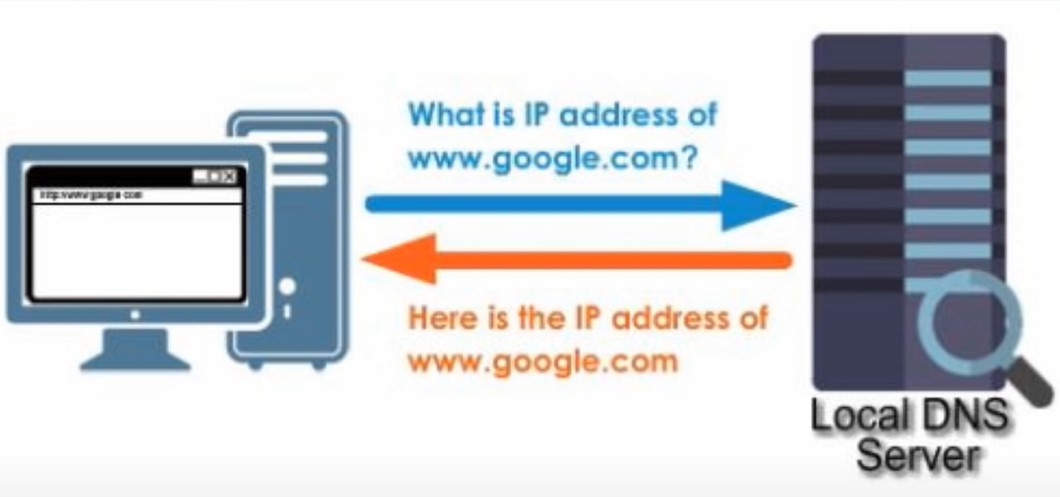
\includegraphics[width=.5\textwidth]{images/dns_recursive_query.jpg}
    \caption[DNS Recursive Query]{Ein Recursive-Query findet zwischen dem DNS-Client und dem \textbf{lokalen} DNS-Server statt\footnotemark[4]}
    \end{center}
\end{figure}
\columnbreak
\begin{figure}[H]
    \begin{center}
        \label{pic:DNSIterative}
        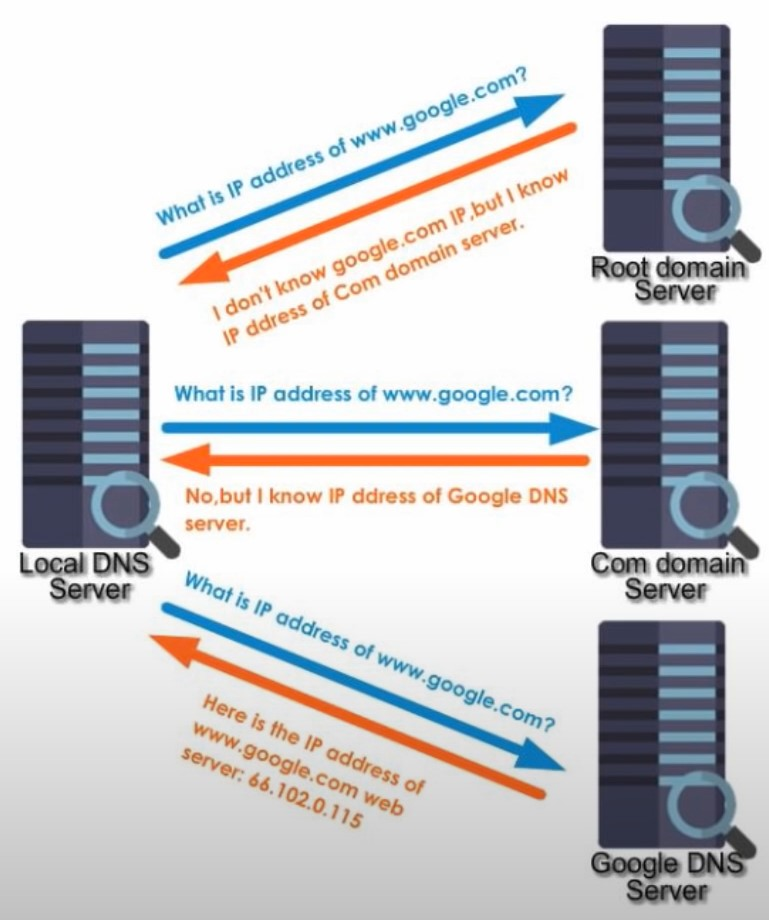
\includegraphics[width=.33\textwidth]{images/dns_iterative_query.jpg}
        \caption[DNS Iterative Query]{Iterative Queries zwischen lokalen DNS-Server und mehreren externen Domain Name Servern\footnotemark[4]}
    \end{center}
\end{figure}
\end{multicols*}

\subsection*{Was für DNS Record Arten gibt es?}\index{DNS!Records}
\begin{itemize}
        \item CNAME
        \item A
        \item AAAA
        \item MX Record
        \item TXT
        \item SRV
\end{itemize}

\subsection*{Was ist die Topologie des DNS Systems? Ist es zentralisiert?}\index{DNS!Topologie}
Es ist verteilt, verschiedene Server haben Zugriff.

\subsection*{Wie kann ich direkt eine DNS Anfrage aus meinem Computer ausführen?}\index{DNS}
Mittels NS Lookup kann man die IP oder Domain eines bestimmten Computers herausfinden.

\subsection*{Was sind die Sicherheitsmerkmale von DNS?}\index{DNS!Sicherheit}
DNS kennt nur System innerhalb des Netzwerks. Initial wurden keine Sicherheitsmechanismen eingebaut. Diese wird gewährleistet durch die Anbieter, z. B. von CloudFlare. Diese bieten Schutz vor DDoS-Attacken, DNS-Spoofing etc. an.

\subsection*{Was für Sicherheitserweiterungen gibt es für DNS?}\index{DNS!Sicherheit!Erweiterung}
Domain Name System Security Extensions (DNSSEC) DNSSEC verhindert, dass Angreifer die Antworten auf DNS-Anfragen verfälschen oder manipulieren.

\subsection*{Wie geht DNS mit den verschiedenen IP Versionen um?}\index{DNS!IP-Version}
\begin{itemize}
    \item A für ipv4
    \item AAAA für ipv6
\end{itemize}

\section{Antworten T2}
\subsection*{Wie erhält ein Host seine IPv4 Konfiguration mit DHCP?}\index{DHCP}
\begin{itemize}
    \item DHCP oder \flqq{}Dynamic Host Configuration Protocol\frqq wird in der Netzwerktechnik verwendet, um einem Client alle nötigen Netzwerkinformationen zuzuweisen, wie:
    \begin{itemize}
        \item IP-Adresse
        \item Subnetzmaske
        \item Standardgateway
        \item Domain Name Server (DNS)
    \end{itemize}
    \item Es können mehrere DHCP Server in einem Netzwerk vorhanden sein, dies ist für die Availability des Services von Vorteil, sollte ein DHCP Server Probleme aufweisen
    \item Discover-Offer-Request-Acknowledgement (DORA)
    \begin{itemize}
        \item DHCP Discover als Broadcast
        \item DHCP Offer
        \begin{itemize}
            \item Mit Client MAC, IP, Subnetz, Gateway, Leasttime und IP des DHCP
        \end{itemize}
        \item DHCP Request als Broadcast
        \begin{itemize}
            \item Annahme der IP Daten
        \end{itemize}
        \item DHCP Acknowledgment
        \begin{itemize}
            \item Bestätigung mit weiteren Optionen
        \end{itemize}
    \end{itemize}
\end{itemize}

\subsection*{Welche Nachrichten des DHCP Protokolls sind Broadcasts und wieso?}\index{DHCP}
\begin{itemize}
    \item Discover, weil er das Netzwerk noch nicht kennt und die IP des DHCP Servers braucht
    \item Request, weil alle im Netz wissen müssen, dass diese IP nun vergeben wurde
\end{itemize}

\subsection*{Was passiert, wenn mehr als ein DHCP Server in dem lokalen Netzwerk verfügbar ist? Ist das möglich? Ist das wünschenswert?}
\begin{itemize}
    \item Hat man mehrere DHCP Server im Netz, gibt es mehrere Offers
    \item Mittels Request der als Broadcast fungiert werden alle DHCP Servers darüber informiert, dass der Client diese gewählt hat
\end{itemize}

\subsection*{Welche Parameter werden typischerweise von einem DHCP Server vergeben?}\index{DHCP!Parameter}
IP, Subnetz, Standardgateway

\subsection*{Was macht ein Host, wenn er keine IPv4 Konfiguration via DHCP bekommt? Kann er mit anderen Hosts kommunizieren?}\index{DHCP!Link-Local}\index{Link-Local}
\begin{itemize}
    \item Werden keine statischen IP-Adressen an einen Client vergeben, weisen sich die Clients bei einem Ausfall vom DHCP automatisch eine IP-Adresse in folgenden IP-Range zu: 169.254.0.0 - 169.254.255.255.
    \item Diese sogenannten Link-Local Adressen ermöglichen eine Kommunikation in einem gemeinsamen lokalen Netzwerk
\end{itemize}

\subsection*{Wie erhält ein Host seine IPv6 Konfiguration mit DHCPv6?}\index{DHCP!IPv6}
Für DHCPv6 gibt es zwei verschiedene Verfahren:
\begin{itemize}
    \item \textbf{Stateless Config:} Router verteilt die IPv6 Präfix und der DHCPv6 die restlichen Parameter
    \item \textbf{Statefull Config:} Der DHCPv6 verteilt IPv6 Präfix als auch die restlichen Parameter Für IPv6 wird das Protokoll DHCPv6 benützt
\end{itemize}

\section{Antworten T3}
\subsection*{Wie wird ein E-Mail mit SMTP verschickt (end-to-end)?}\index{SMTP}
SMTP - Simple Mail Transfer Protocol gehört zur Anwendungsschicht, bedeutet Simple Mail Transfer Protocol und dient, wie der Name sagt, zum Austauschen von E-Mails. SMTP funktioniert über \textbf{TCP}. Kann auch als Gedankenstütze mit Sending-Mail-To-People genutzt werden.\\[1em]
Schritte:
\begin{enumerate}
    \item Ein Mail-Client (Outlook) sendet E-Mail an SMTP Server.
    \begin{itemize}
        \item Wenn Gmail genutzt wird, ist dieser Server smtp.gmail.com
    \end{itemize}
    \item Dieser SMTP-Server sendet dann die Mail an den SMTP Server des Empfängers.
    \item E-Mail wird vom SMTP Server des Empfängers erhalten.
    \item Hier endet das SMTP. Um die E-Mails abzurufen, kommen dann IMAP/POP3 zum tragen.
\end{enumerate}

\subsection*{Wie wird der Nutzer des SMTP Servers authentifiziert?}\index{SMTP!Authentifizierung}
\begin{itemize}
    \item Authentifizierung: Beispiel mit Brief Absenderadresse, die vom Versender angepasst werden kann. Dies soll verhindert werden mit SMTP.
    \item SMTP Auth ist Extension von Extended SMTP was wiederum eine Erweiterung von SMTP ist.
    \item Somit können nur noch Vertrauenswürdige Nutzer Emails über diesen Sender Server versenden.
    \item Statt über den Standardport 25/TCP wird über den Port 587 kommuniziert. Obligatorische Grundlage für E SMTP. Verschiedene Authentifizierungsmechanismen (PLAIN, LOGIN, CRAM-MD5).
\end{itemize}

\pagebreak
\subsection*{Welche Sicherheitseigenschaften hat SMTP? Was für Sicherheitserweiterungen gibt es?}\index{SMTP!Sicherheit!Erweiterung}
Eine Vertraulichkeit, Authentizität und Integrität von E-Mails kann durch SMTP allein nicht gewährleistet werden. Clientseitige Verfahren müssen genutzt werden. Ansonsten sind die Absender und Empfänger fälschbar und die E-Mailinhalte grundsätzlich lesbar und veränderbar.
\begin{itemize}
    \item \textbf{S/MIME} ist eine Technologie, die \textbf{E-Mails verschlüsselt}, um sie vor unerwünschtem Zugriff zu schützen. Ausserdem können die \textbf{E-Mails digital signiert} werden, um den Absender als legitim zu verifizieren.
    \begin{itemize}
        \item Zugemüse: Meistens sind S/MIME-Zertifikate kostenpflichtig, da sie als Paket auf Corporate-Level angeboten werden. Actalis\footnote{\url{https://extrassl.actalis.it/portal/uapub/freemail?lang=en}} ist eine Root Certificate Authority und bietet kostenlose Zertifikate für eine Mail-Adresse für je ein Jahr aus, welche man jeweils erneuern kann.
    \end{itemize}
    \item \textbf{PGP (Pretty Good Privacy)} ist eine alternative Methode E-Mails zu signieren und verschlüsseln. Anders als S/MIME, wo eine Root Certificate Authority Zertifikate ausstellt, basiert PGP auf ein Web of Trust.
    \begin{itemize}
        \item Zugemüse: Wer sich interessiert, kann hier eine Infografik\footnote{\url{https://emailselfdefense.fsf.org/en/infographic.html}} anschauen und hier eine einfache Anleitung\footnote{\url{https://emailselfdefense.fsf.org/en/index.html}} lesen, um PGP bei sich aufzusetzen. GPG4Win\footnote{\url{https://www.gpg4win.org/}} bietet mit Kleopatra eine benutzerfreundliche Oberfläche zum erstellen und verwalten seiner Schlüssel (auch S/MIME).
    \end{itemize}
    \item \textbf{TLS}: Verschlüsselt die Verbindung und Daten während der Übertragung von Punkt A nach Punkt B. Der Schlüsselaustausch findet im Hintergrund statt, ohne Einwirken des Benutzers.
\end{itemize}

\subsection*{Kriegt die Empfängerin das E-Mail sobald es von dem SMTP Server empfangen wird?}\index{SMTP!Empfang}
Wenn ein Server eine Nachricht erhält, legt er die Nachricht entweder lokal ab oder leitet sie einem anderen E-Mail-Server weiter. Ist der Destination E-Mail-Server nicht online, oder beschäftigt, so sendet SMTP die Nachricht zu einem späteren Zeitpunkt. Wenn sie nach einer bestimmten Zeit immer noch nicht zugestellt werden kann, dann wird sie dem Sender als unzustellbar zurückgeschickt.

\subsection*{Wie wird auf E-Mails mit POP3 zugegriffen?}\index{POP3}
POP3 - Post Office Protocol Version 3 ist das Übertragungsprotokoll für E-Mails und stammt aus dem Jahr 1996. Dabei verbindet sich der POP3 Client mit dem Mailserver und authentifiziert sich durch ein \textbf{Passwort}. Sodann ruft der Client neue Nachrichten für die Mailadresse ab und der Server sendet diese E-Mails an den Client. Nach der Übertragung löscht der Server die Nachrichten.

\subsection*{Wie wird auf E-Mails mit IMAP zugegriffen?}\index{IMAP}
Bei IMAP - Internet Message Access Protocol basierten Mailclients werden die Mails sowie die Ordnerstrukturen und Einstellungen auf einem Mailserver gespeichert. Der Client holt sich dann die einzelnen Informationen erst vom Server, wenn sie gebraucht werden. Eine normale IMAP Kommunikation beginnt mit einem \textbf{Login}, wobei sich der Client mit einem \textbf{Username} und einem \textbf{Password} beim Mailserver authentifiziert. Danach kann der Client dem Server diverse Anfragen stellen, um Infos über die Mails zu bekommen oder um die Mails auf dem Server zu bearbeiten (verschieben, löschen, markieren, etc.)

\subsection*{Was sind die Hauptunterschiede zwischen POP3 und IMAP? Wann wird es empfohlen sie zu verwenden? }
Beim POP3 werden die Daten lokal abgespeichert und auf dem Server gelöscht. Mit dem IMAP ruft der Client die Daten vom Server ab. Möchte man \textbf{wenig Bandbreite} nutzen, sollte man \textbf{POP3} verwenden. Will man mit \textbf{mehreren Devices} auf die Mails zugreifen und ein sicheres Backup haben, empfiehlt es sich das \textbf{IMAP} zu verwenden.

\pagebreak
\section{Antworten T4}
\subsection*{Wie wird auf eine Website mit HTTP(S) zugegriffen?}\index{HTTP(S)}
Nach der DNS-Auflösung wird mit der GET Methode von HTTP(s) auf Webseite über den Port 80 (443 bei HTTPS) zugegriffen. Wird diese GET Anfrage vom Webserver akzeptiert, so sendet er erst Inhalt des Headers des Bereitgestellten HTML Dokuments und im Anschluss den Body. Der Body repräsentiert den Inhalt einer Webseite und ist das, was der User im Interface seines Webbrowsers sieht. Im Anschluss wird die Verbindung beendet.

\subsection*{Was ist der Unterschied zwischen HTTP und HTTPS?}\index{HTTP(S)}
Das "`S"' von HTTPS steht für Secure. Bei einer HTTPS Verbindung wird das Webbrowser Zertifikat zum Verschlüsseln der Verbindung verwendet. Somit ist die Verbindung über SSL/TLS (Transport Layer Security) gesichert und die gesendeten Daten, können nicht oder nur schwer abgehört werden. HTTPS ist heutzutage beinahe ein \textsl{de facto} Standard für alle offiziellen Webseiten.

\subsection*{Was sind die Hauptmerkmale von TLS? Wie funktioniert TLS (hohes Niveau)?}\index{TLS}
TLS (Transport Layer Security) ist ein Protokoll der 5 Schicht, welches zuständig ist für eine sichere Datenübertragung im Internet. Nebst dem HTTPS Protokoll können auch Protokolle wie SMTP, FTP, POP3, etc. das TLS Protokoll verwenden. Die Funktion ist in \textbf{zwei Phasen} unterteilt: Die \textbf{erste Phase} ist der \textbf{Verbindungsaufbau} und die \textbf{zweite Phase} ist die \textbf{Übermittlung}.\\[1em]

Es wird mit zwei verschiedenen Schlüsseln gearbeitet (Private und Public Key).
\begin{itemize}
    \item Der Public Key vom Empfänger ist jeweils dem Sender bekannt.
    \item Mit dem Public Key werden Daten verschlüsselt und mit dem Private Key werden die Daten entschlüsselt.
    \item Bevor die Verschlüsselung startet, wird überprüft, ob der Empfänger den echten öffentlichen Schlüssel mitteilt. Die Überprüfung findet mit Hilfe von den Zertifikaten statt.
\end{itemize}

\subsection*{Was sind andere wichtige Verwendungen von HTTP (ausser Websites zuzugreifen)?}\index{HTTP(S)!REST API}
Rest API $\rightarrow$ Schnittstellen bzw. Webservices verwenden HTTP.

\subsection*{Was ist ein REST API?}\index{REST API}
\begin{itemize}
    \item REST - Representational State Transfer
    \item API - Application Programming Interface $\rightarrow$ Programmierschnittstelle, die den Austausch von Informationen ermöglicht, wenn diese sich auf unterschiedlichen Systemen befinden.
\end{itemize}
REST ist ein Software-Architektur-Stil der anleitet, wie internetbasierte Systeme sich zu verhalten haben. Beispielsweise welche Standards, wie JSON oder XML, sich wie zu verhalten haben und wie Daten über HTTP-Methoden auszutauschen sind etc. Die API bietet den Zugang zu den Ressourcen.

\subsection*{Was sind die Hauptmethoden von HTTP?}\index{HTTP(S)!Methoden}
GET, POST, PUT, DELETE, HEAD, CONNECT, OPTIONS, TRACE

\subsection*{Wie funktioniert ein REST API?}\index{REST API}
Die REST Schnittstelle nutzt HTTP-Anfragen, um mit GET, POST, PUT und DELETE auf Informationen zuzugreifen. Jede URL wird als Anforderung bezeichnet, während die zurückgegeben Daten die Antwort sind. Sobald eine Client-Anfrage auf dem Server eingegangen ist, sucht die REST-API nach einer Antwort und liefert sie unverzüglich.

\subsection*{Nenne ein Beispiel von einem REST API Endpoint, der die GET Methode verwendet.}\index{REST API}
Aufrufen einer Ressource $\rightarrow$ Bsp: Facebook Profil aufrufen

\subsection*{Nenne ein Beispiel von einem REST API Endpoint, der die POST Methode verwendet.}\index{REST API}
Anlegen einer Ressource $\rightarrow$ Bsp: Facebook Account erstellen

\subsection*{Nenne ein Beispiel von einem REST API Endpoint, der die PUT Methode verwendet.}\index{REST API}
Verändern einer Ressource $\rightarrow$ Bsp: Facebook status ändern

\pagebreak
\section{Antworten T5}
\subsection*{Wofür wird SSH verwendet?}\index{SSH}
Secure Shell (SSH) bezeichnet ein Protokoll, in welchem Clients auf entfernte Hosts zugreifen können. Administratoren können damit beispielsweise einen Computer durch Fernzugriff konfigurieren und betreuen. Wie der Name "`Shell"' bereits andeutet, ist die GUI eine textbasierte Kommando-Konsole. Die Shell selbst ist ein Kommando-Übersetzer und gibt Instruktionen an den Betriebssystem-Kern (Kernel) weiter.

\subsection*{Wie funktioniert SSH (hohes Niveau)?}\index{SSH}
SSH gibt es standardmässig auf Linux. Neue Windowsversionen, wie Windows 11 und Windows 10 ab Update 1809, bieten einen SSH-Server auf Basis von OpenSSH.
Verbindung mit SSH benötigt IMMER zwei Programme:
\begin{itemize}
    \item Server wie z.B. OpenSSH Server auf entferntem Computer
    \item Client wie SSH (Linux) oder PuTTY (Windows) auf lokalem Rechner
\end{itemize}
Ablauf:
\begin{enumerate}
    \item Verbindungsaufbau zum Server via Hostname, Domain oder IP
    \item Wird Anfrage entgegengenommen, muss Nutzer mit Namen \& Passwort oder durch digitales Zertifikat identifizieren
    \item Dann steht textbasierte Umgebung (Shell) auf Server zur Verfügung und es kann gearbeitet werden
\end{enumerate}
\begin{figure}[H]
    \begin{center}
    \label{pic:SSH}
    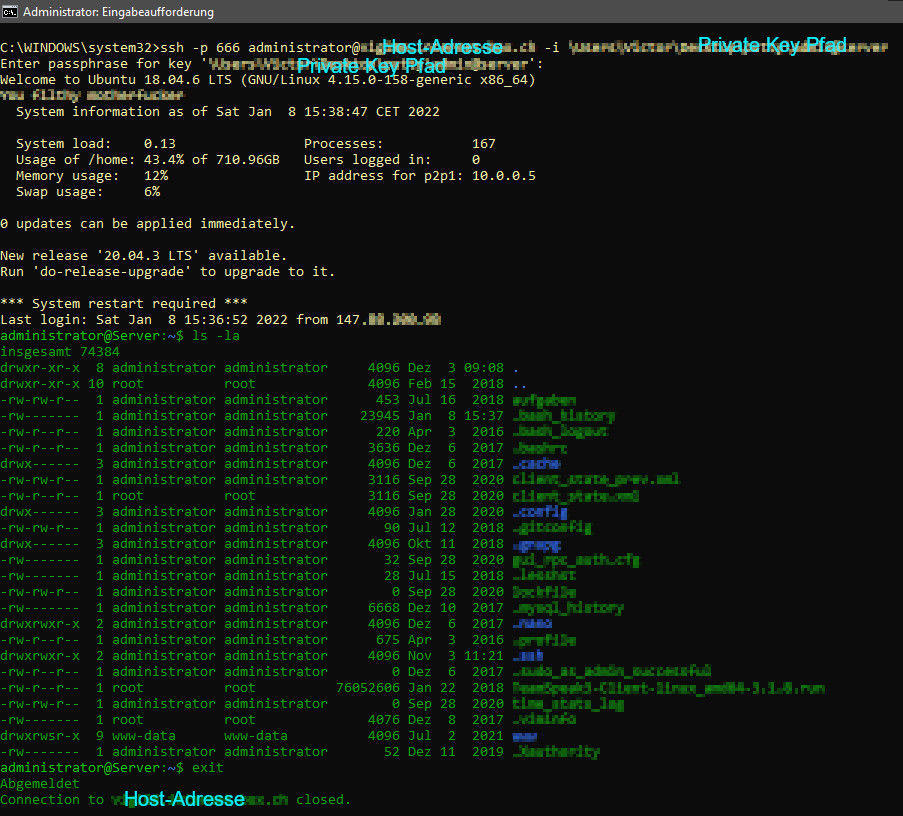
\includegraphics[width=\textwidth]{images/ssh.jpg}
    \caption{SSH von cmd.exe zu Linux-Server}
    \end{center}
\end{figure}

\subsection*{Was für Nutzerauthentifizierungsoptionen gibt es? Was wird empfohlen?}\index{Authentifizierung}
\begin{itemize}
    \item SSH
    \item 2-Factor-Authentication / Multi-Factor-Authentication (MFA)
    \begin{itemize}
        \item Passwort und Email/SMS Code
        \item Doppelte Sicherheit
    \end{itemize}
    \item External Keys
    \item OAuth - Open Standard Authorization Protocol
    \begin{itemize}
        \item Open Authorization ist der Name zweier verschiedener offener Protokolle, die eine standardisierte, sichere API-Autorisierung für Desktop-, Web- und Mobile-Anwendungen erlauben. Ein User kann mit Hilfe dieses Protokolls einer Anwendung den Zugriff auf seine Daten erlauben (Autorisierung), die von einem anderen Dienst bereitgestellt werden, ohne geheime Details seiner Zugangsberechtigung (Authentifizierung) dem Client preiszugeben. Der User kann so Dritten gestatten, in seinem Namen einen Dienst zu benutzen. Typischerweise wird dabei die Übermittlung von Passwörtern an Dritte vermieden.\cite{wiki}
    \end{itemize}
    \item SAML - Security Assertion Markup Language
    \begin{itemize}
        \item Dia SAML ist ein XML-Framework zum Austausch von Authentifizierungs- und Autorisierungsinformationen. Sie stellt Funktionen bereit, um sicherheitsbezogene Informationen zu beschreiben und zu übertragen.
        \begin{itemize}
            \item Single Sign-On - ein Benutzer ist nach der Anmeldung an einer Webanwendung automatisch auch zur Benutzung weiterer Anwendungen authentifiziert
            \item Verteilte Transaktionen – mehrere Benutzer arbeiten gemeinsam an einer Transaktion und teilen sich die Sicherheitsinformationen
            \item Autorisierungsdienste – die Kommunikation mit einem Dienst läuft über eine Zwischenstation, die die Berechtigung überprüft
        \end{itemize}
    \end{itemize}
\end{itemize}

\subsection*{Was ist RDP?}\index{RDP}\index{Remotedesktop!RDP}
RDP - Remote Desktop Protocol ermöglicht den Zugriff auf einen entfernten Desktop.

\subsection*{Wie funktioniert RDP?}\index{RDP}\index{Remotedesktop!RDP}
User kann Aktionen auf dem entfernten Computer als Terminal durchführen. RDP öffnet einen dedizierten Kanal zwischen zwei Verbundenen Geräten und nutzt immer Port 3389. Via TCP/IP werden die Kommandos ausgetauscht.. RDP verschlüsselt alle Daten, damit die Verbindung noch sicherer ist.

\subsection*{Was ist VNC?}\index{VNC}\index{Remotedesktop!VNC}
VNC - Virtual Network Computing wird im übergeordneten als Remote Desktop Sharing bezeichnet. User können damit den Computer aus dem Geschäft zuhause anzeigen lassen.

\subsection*{Wie funktioniert VNC?}\index{VNC}\index{Remotedesktop!VNC}
\begin{itemize}
    \item Funktioniert im Client-Server Modell
    \item User muss nur einen VNC Viewer auf einem lokalen Computer (client) haben. Dieser verbindet sich von entfernt auf einen anderen Computer, wo VNC als Server installiert ist.
    \item VNC ist Plattformunabhängig, beide Computer müssen lediglich TCP/IP aktiviert haben und offene Standard-Ports (TCP 5800, 5900) mit zugelassenem Traffic.
\end{itemize}

\subsection*{(Zusätzlich) Was ist der Unterschied zwischen RDP und VNC?\footnote{\url{https://www.parallels.com/blogs/ras/vnc-vs-rdp/}}}\index{RDP}\index{Remotedesktop!RDP}\index{VNC}\index{Remotedesktop!VNC}
\begin{itemize}
    \item Grundsätzlich: zwei verschiedene Protokolle
    \begin{itemize}
        \item RDP: \flqq{}Client zu Client\frqq
        \item VNC: \flqq{}Client zu Server\frqq
    \end{itemize}
    \item RDP ist schneller und eignet sich für Virtualisierung besser
    \item RDP unterstützt SSL/TLS und bekommt Security Updates
    \item Nicht jede VNC Software akzeptiert SSH, VNC gibt den Clients \flqq{}Full Access\frqq
\end{itemize}

\subsection*{Was ist VDI?}\index{VDI}\index{Remotedesktop!VDI}
Die VDI - Virtual Desktop Infrastructure sorgt dafür, dass ein Geschäftscomputer von überall her zugreifbar ist.

\subsection*{Wie funktioniert VDI?\footnote{\url{https://azure.microsoft.com}}}\index{VDI}\index{Remotedesktop!VDI}
\begin{itemize}
    \item Komplexer als einfache RDP weil noch Server etc. virtualisiert drinnen mithängen.
    \item Desktop OS ist meisten in einem Zentralisierten Server oder einem physischen Datencenter gehostet.
    \item Es gibt zwei Arten:
    \begin{itemize}
        \item Persistent Virtual Desktop - Speichern für Zukünftige Nutzung, traditioneller Desktop
        \item NonPersistent - Einheitliche Desktops, wo man auf das zugreifen kann, was man braucht. Desktop geht zurück in Einheitlichen Status nachdem der User sich ausloggt
    \end{itemize}
\end{itemize}

\subsection*{Nenne Beispiele von kommerziellen VDI Lösungen}\index{VDI}\index{Remotedesktop!VDI}
\begin{itemize}
    \item Citrix Workspace
    \item VirtualBox
    \item VM Fusion
    \item Amazon WorkSpaces
\end{itemize}
